\chapter{Results and Evaluation}
\label{chapter:results-and-evaluation}

This chapter will focus on the data obtained in the project. For clarity, there is a separate section on each fractal, as they are quite different and had their own sets of representative views. A small explanation of the expected results will be given for each fractal. For the temporal caching, there were some tests that could be performed, that could not be performed with the signed distance field, because they involved animations that either changed the geometry or travelled far outside acceptable range for the signed distance field. Therefore, static image tests will be separated from animation tests. After each set of results is presented, discussion and evaluation of those results will be done.\newline

The unoptimized time given is the time taken to execute the entire geometry render pass, in nanoseconds. The performance gain (or loss) is measured by obtaining the percentage difference between the unoptimized method, and the optimized one, like so:

\begin{equation}
	diff = \frac{unopt - opt}{unopt} * 100
\end{equation}

where unopt and opt are the unoptimized time and optimized time, respectively.

\section{Mandelbulb Static Image Tests}

\subsection{Representative Views}

\begin{figure}[ht]
	\centering

	\begin{subfigure}[c]{0.45\linewidth}
		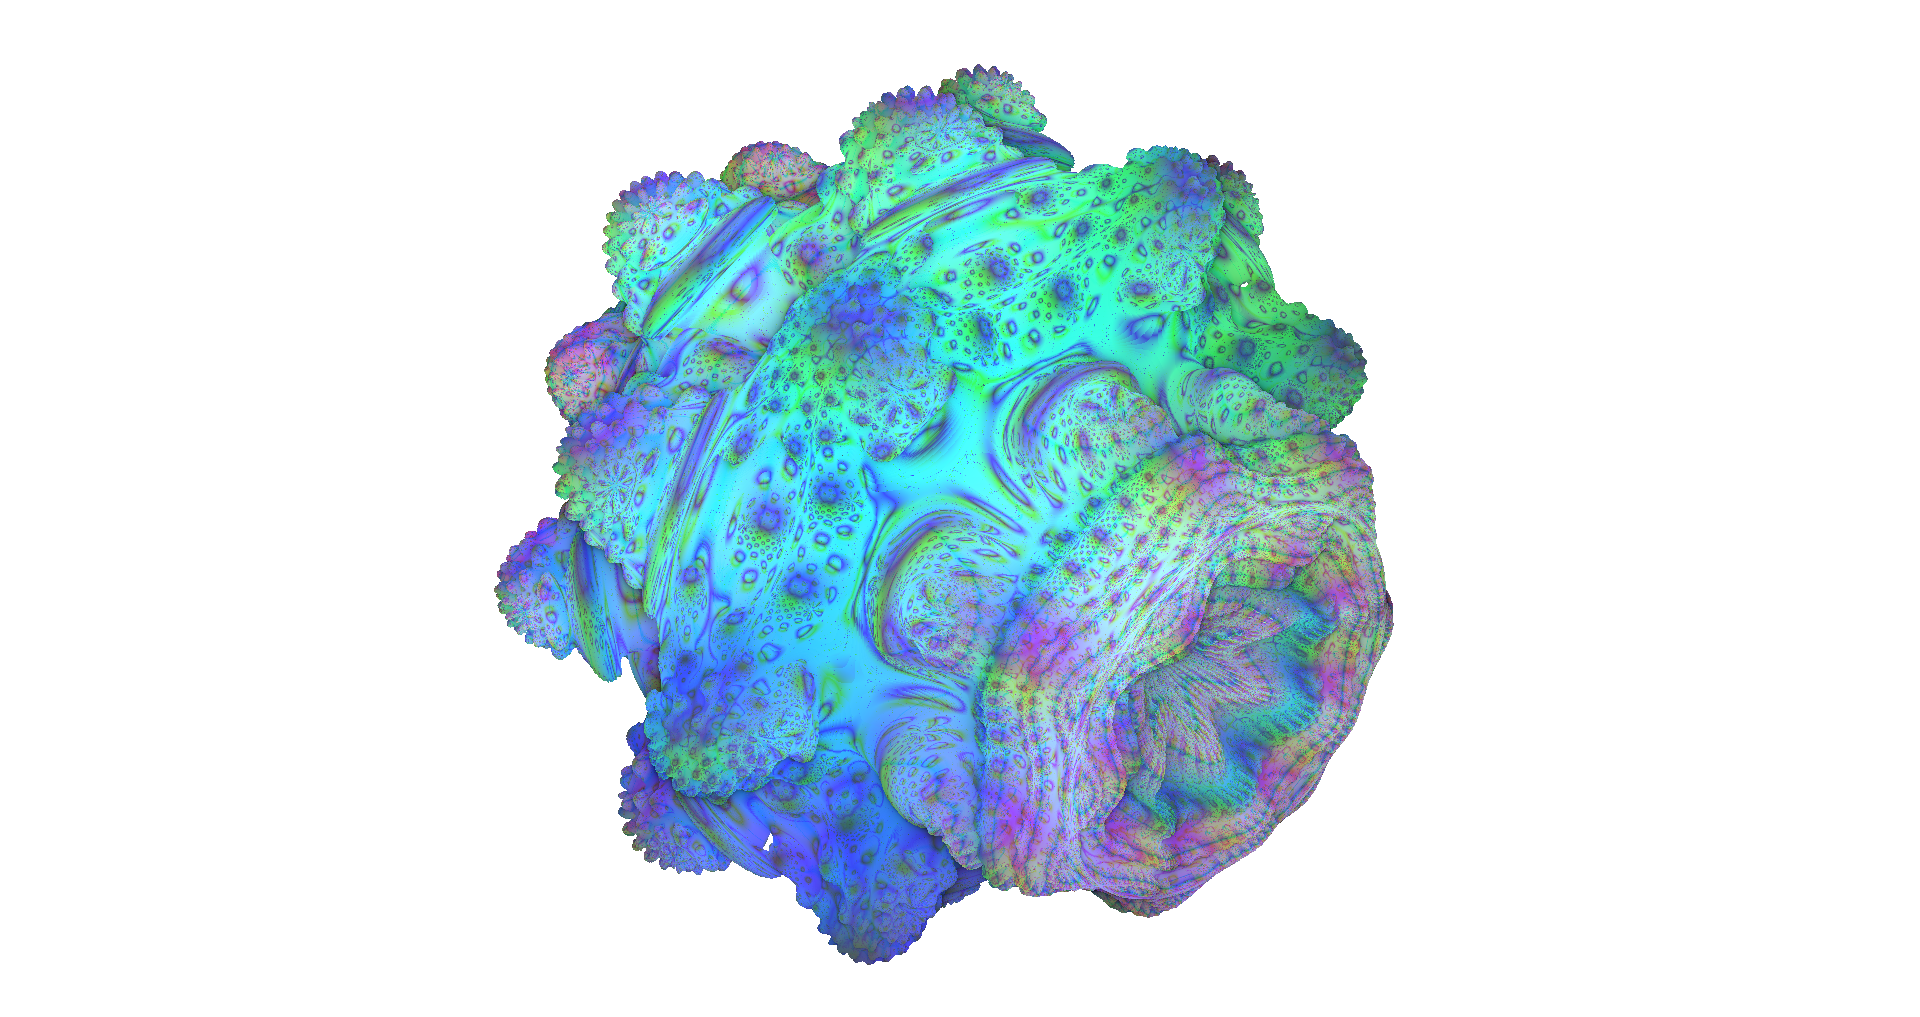
\includegraphics[width=\linewidth, frame]{Images/Results/Mandelbulb-View-01-Default.png}
		\caption{Mandelbulb: Default View.}
		\label{figure:mandelbulb-view-01-default}
	\end{subfigure}
	\hfill
	\begin{subfigure}[c]{0.45\linewidth}
		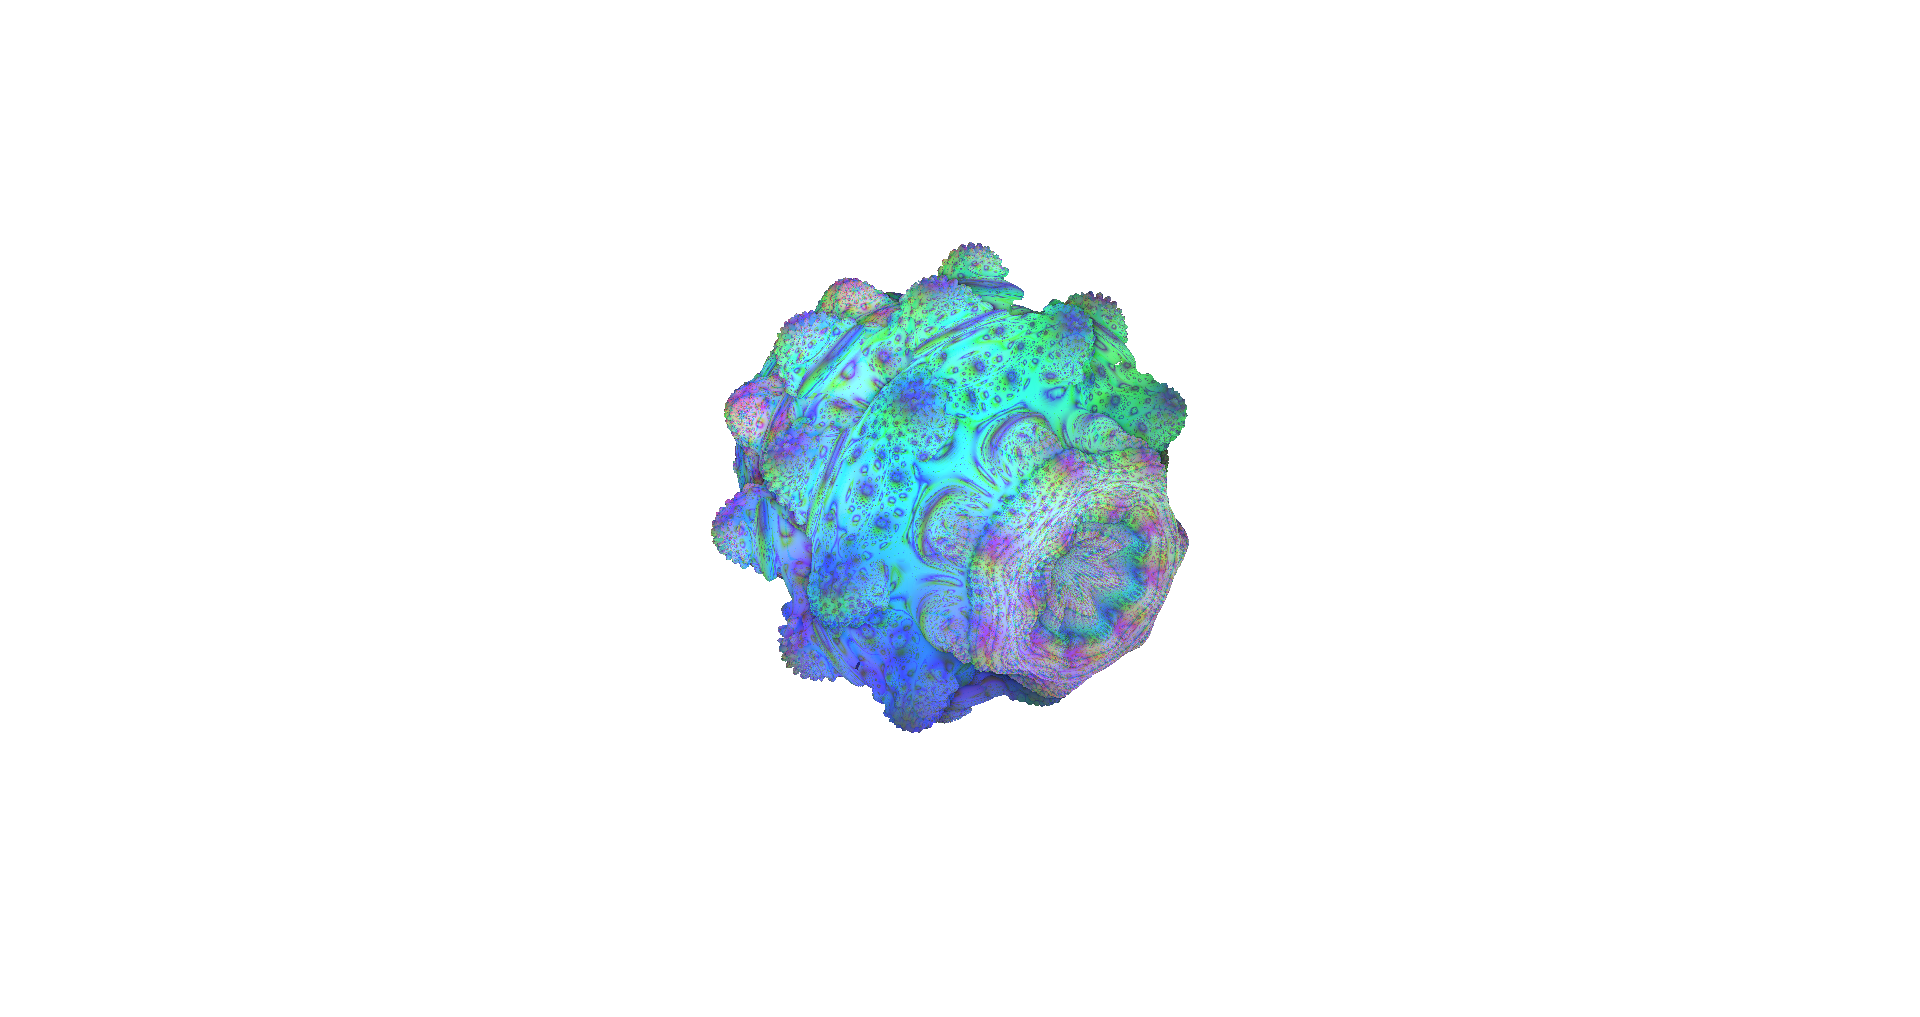
\includegraphics[width=\linewidth, frame]{Images/Results/Mandelbulb-View-02-Empty-Space.png}
		\caption{Mandelbulb: Zoomed Out View.}
		\label{figure:mandelbulb-view-02-empty-space}
	\end{subfigure}
	\hfill
	\begin{subfigure}[c]{0.45\linewidth}
		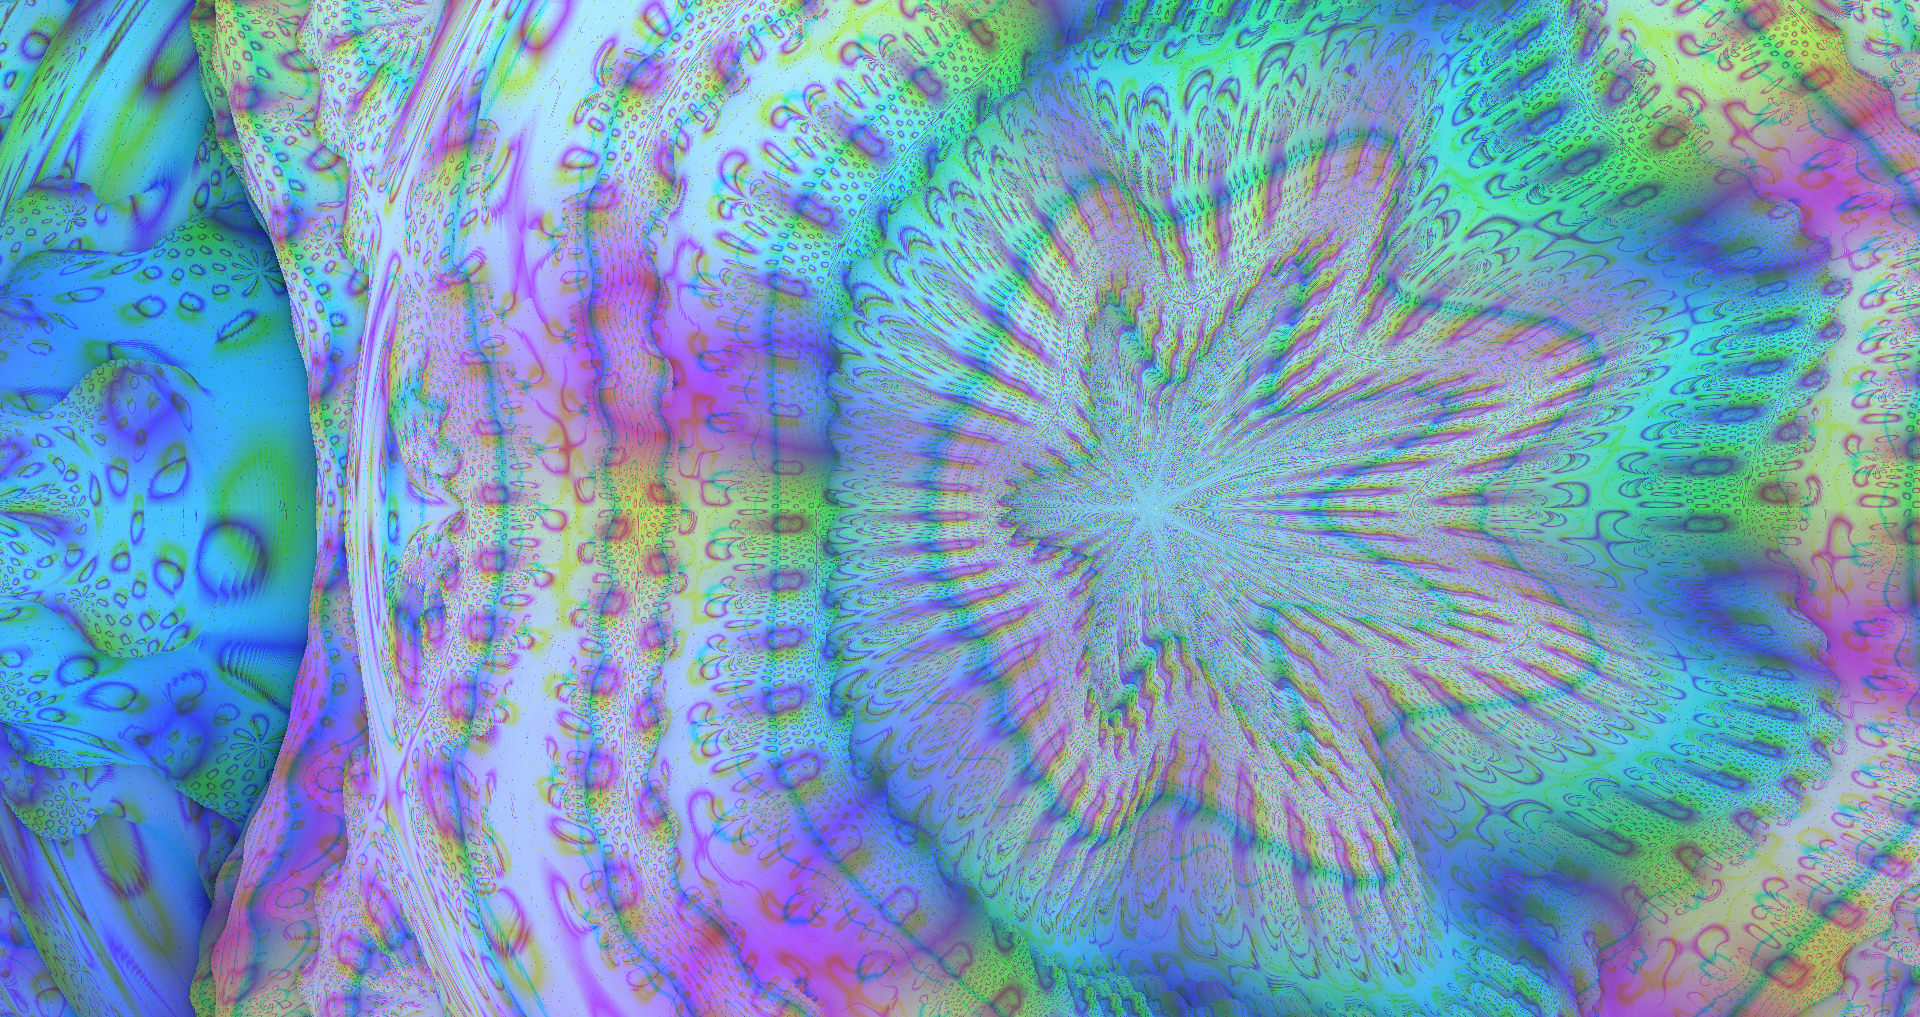
\includegraphics[width=\linewidth, frame]{Images/Results/Mandelbulb-View-03-No-Space.png}
		\caption{Mandelbulb: Zoomed In View.}
		\label{figure:mandelbulb-view-03-no-space}
	\end{subfigure}
	\hfill
	\begin{subfigure}[c]{0.45\linewidth}
		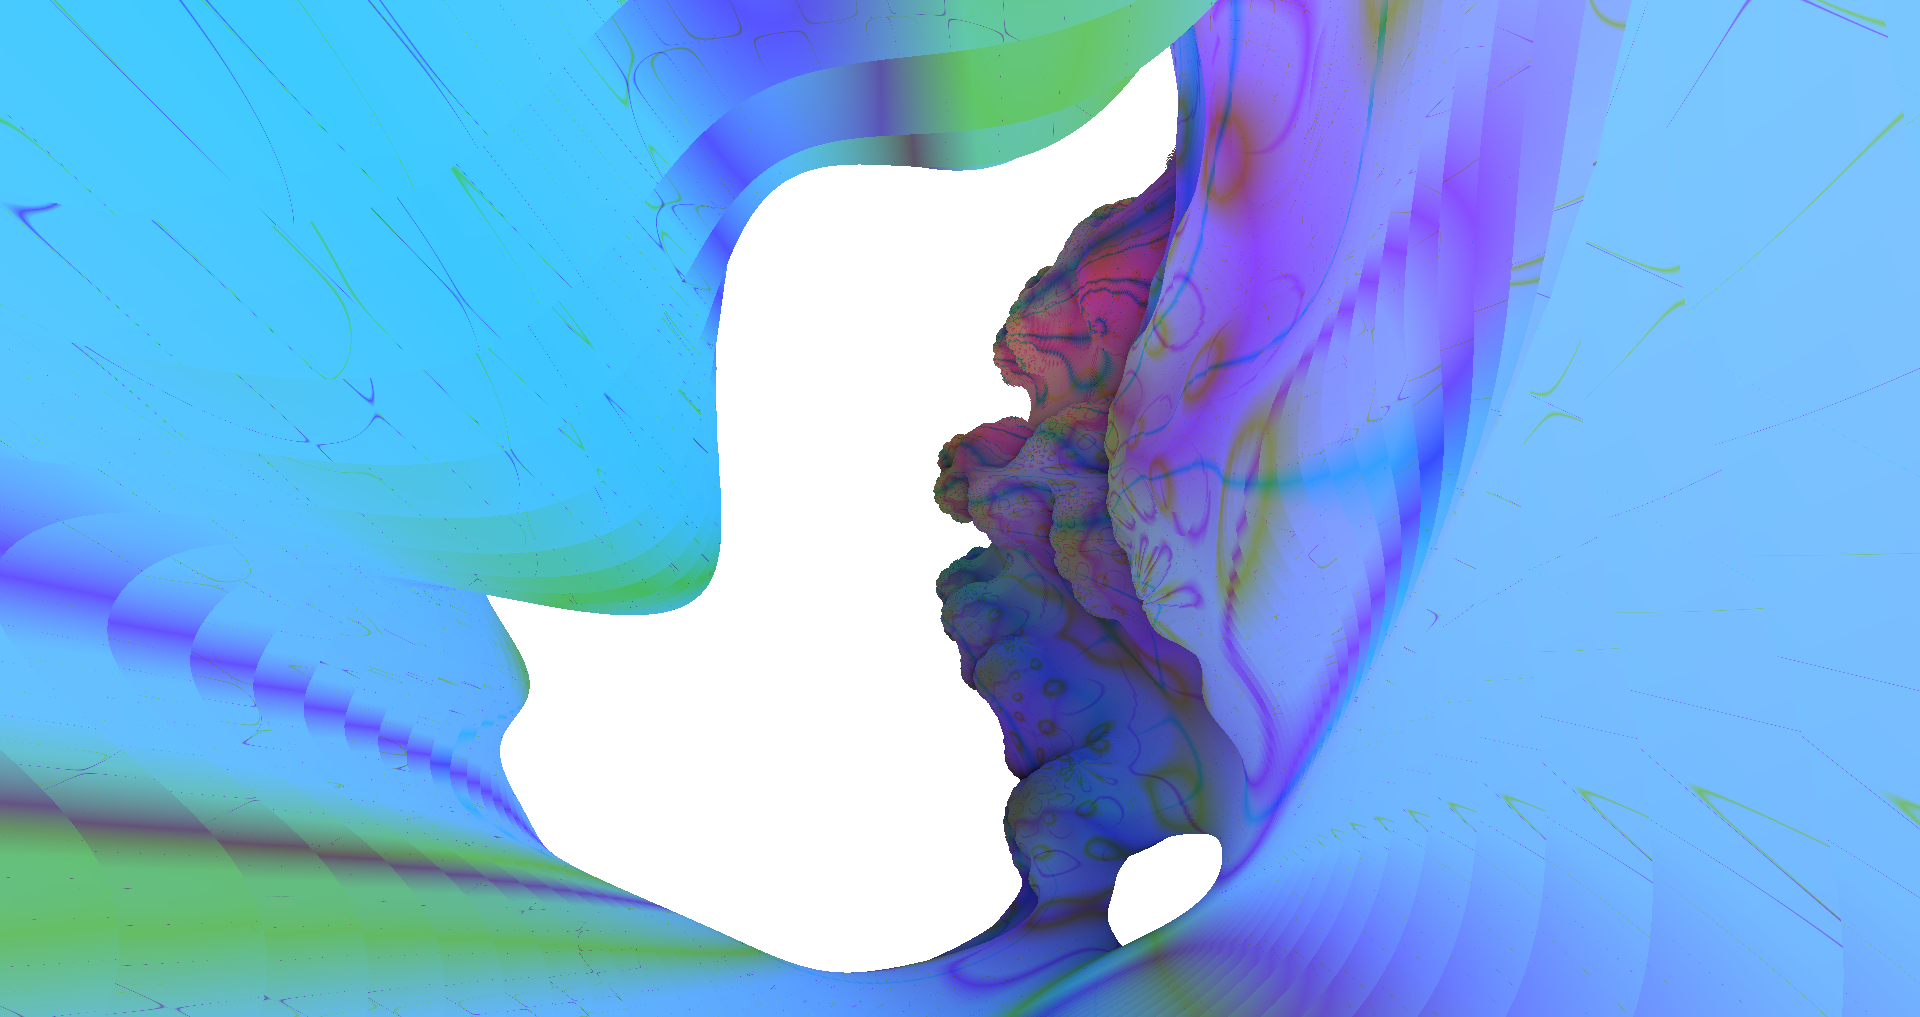
\includegraphics[width=\linewidth, frame]{Images/Results/Mandelbulb-View-04-Bottleneck.png}
		\caption{Mandelbulb: Bottleneck View.}
		\label{figure:mandelbulb-view-04-bottleneck}
	\end{subfigure}

	\caption{Four representative views of the Mandelbulb fractal, used in performance tests.}
	\label{figure:mandelbulb-views}
\end{figure}

Figure \ref{figure:mandelbulb-views} shows the four representative views used for performance measurements. Figure \ref{figure:mandelbulb-view-01-default} shows the default view, which is not expected to be particularly well suited to any performance measurement, to get a general-case overview of the performance differences between the methods used. Figure \ref{figure:mandelbulb-view-02-empty-space} is the view intended to include the most empty space (short of simply turning around and not looking at the fractal at all), and by contrast figure \ref{figure:mandelbulb-view-03-no-space} is intended to include the least. Lastly, figure \ref{figure:mandelbulb-view-04-bottleneck} includes a mix of depth and smoothness, and some bottlenecks.

\subsection{Expected Results}

The view of the Mandelbulb fractal involves quite a bit of empty space, unlike the Hall of Pillars fractal, which contains none. The expected result is that the Temporal caching method will give a slight performance boost to views with empty space, especially around the edges of the fractal, where more iterations would normally occur, but huge boosts are not expected since the Mandelbulb does not contain so many bottlenecks, and the depth variance is small. For still images, though, the temporal caching should give a boost no matter what is being looked at, as long as the camera does not move.\newline

For the signed distance field, it entirely depends on whether searching through the three-dimensional grid is less expensive than calculating the signed distance function or not, as the signed distance field is intended to provide a cheaper alternative every iteration, not to reduce the number of iterations as the temporal caching is supposed to do. The prediction is that the more costly the function, the more benefit will be seen, but that, since the Mandelbulb function is relatively cheap, there won't be much benefit, if any, with the distance function used here.

\subsection{Results}

\begin{table}[ht]
	\centering
	\begin{tabular}{||p{0.2\linewidth}|p{0.29\linewidth}|p{0.23\linewidth}|p{0.23\linewidth}||}
		\hline
		View & Unoptimized Time (ns) & SDF Difference (\%) & TC Difference (\%)\\
		\hline\hline
		Default & 1272832 & -154.38 & 2.06\\
		\hline
		Zoomed Out & 1083328 & -60.08 & 8.67\\
		\hline
		Zoomed In & 1241088 & -33.74 & -2.30\\
		\hline
		Bottleneck & 1593888 & -6.8 & 7.01\\
		\hline
	\end{tabular}
	\caption{A table showing the performance differences between the two optimization methods and the base, unoptimized rendering, for four different views of the Mandelbulb.}
	\label{table:mandelbulb-static-results}
\end{table}

Table \ref{table:mandelbulb-static-results} shows the results obtained for the four representative views of the Mandelbulb fractal. It shows the unoptimized time and the performance differences with the SDF and Temporal Caching (TC).

\subsection{Evaluation}

Following the gathering of results, I decided to do a one-iteration performance measurement. In the shaders, I allowed one iteration of either the SDF search process, or the distance estimation, for the SDF shader and the unoptimized shader, respectively. The result was as expected; the render pass took 0.446ms with no optimizations, and 0.556ms with the SDF.

\subsubsection{Signed Distance Field}

Clearly, the signed distance field did not do well for this fractal, even though at first glance it seems a perfect fit for it, seeing as the whole fractal fits inside a reasonable boundary. I think overall, this is because the distance estimator for the Mandelbulb is so cheap, so the search through the SDF is outpaced by the distance function.\newline

The worst performance is seen with the default view. This may be because the whole fractal is visible, and fairly close to the camera, so fine detail is visible. This means that more iterations are needed, and most of them will fall within the cube, at least at first, making this the worst performer. Contrast that with the zoomed out view, where most of the rays fall outside the boundary of the SDF, which saves the performance a little, as the shader will revert to using the regular signed distance function if this happens. Additionally, less of the fractal is visible here, and in less detail. It seems that the performance measurements for the Mandelbulb simply show which of the views the SDF fights against the least.\newline

The zoomed in view is a little better. Considering the performance of the SDF so far, I think this view is better simply because it is closer to the fractal. This means that less iterations are done before the ray gets close enough to the surface of the fractal to begin using the regular signed distance function. I think the bottleneck view performed the best for a similar reason, with the addition that the surface is even simpler in this view, and the view out to the background is quite close to the edge of the SDF boundary, so it wouldn't be very many iterations once past the bottleneck to be free of the SDF cube.\newline

The SDF is not a suitable optimization for this fractal, in its current state. The process of searching through the SDF is clearly more expensive than the signed distance function calculation. If I were to use a more expensive fractal then maybe using the SDF would be worthwhile.

\subsubsection{Temporal Cache}

The temporal cache performed much better than the SDF, to the point where it actually gives a performance boost. The scenarios are also a little easier to explain. Starting with the zoomed in view, which decreased the performance. The surface in this view is quite detailed, and close to the camera. I think the performance difference was negative because of the deliberate underestimate that happens when using the saved distance. It is multiplied by 0.9, meaning that any iterations in that last 10\% are lost every frame. In this case, I think that most of the iterations happen in this last 10\%, where the surface becomes more complex, so the temporal cache provides no benefit here. The negative difference most likely comes from the overhead involved in sampling from the texture image, and the extra comparisons that happen for the camera movement test, for example.\newline

The largest performance difference came from the zoomed out view. I was expecting it to come from the bottleneck, but I suppose that in terms of edges, the zoomed out view contains just as many. In addition, the empty space will also receive a boost, and not just around the edges, so a large part of the performance increase likely comes from here. As well as this, less of the fractal surface is visible, so although the problem present in the zoomed in view applies, and most of the iterations for the surface come from that last 10\% that is cut out, the portion of the image to which this applies is very small in this view.\newline

The performance for the default view lines up with the explanations for the zoomed out and zoomed in views. There is more empty space, and there are more edges, in the default view than in the zoomed in view, so the performance will be better, but there is also more surface space, which this optimization method does not perform well on, so that will cause a hit to overall performance.\newline

This drawback does not apply so much to the bottleneck scenario, despite it being close to the surface. There is not a lot of complicated geometry in this view, so the cut to iteration progress doesn't hit the performance so hard. Most of the performance boost probably comes from the avoidance of the obvious bottleneck (hole) in the middle, and the smaller one on the right.\newline

Overall, the temporal cache is worth using for the Mandelbulb fractal, just looking at the static views.

\section{Mandelbulb Animation Test}

This section will examine the performance while animating the Mandelbulb by changing its parameter. Recall figure \ref{figure:mandelbulb-powers} in chapter \ref{chapter:implementation}. It shows the Mandelbulb, raised to different powers. This power is the parameter that is varied in the animation.

\subsection{Animation}

The animation of the Mandelbulb parameter takes a total of 8000 frames. The parameter starts at 10 and gets raised to 16 by the end of the first 2000 frames. Then, it decreases to 4 over 4000 frames. Finally, over 2000 frames it returns to 10. Refer back to figure \ref{figure:mandelbulb-powers} in chapter \ref{chapter:implementation} for an overview of how this looks.

\subsection{Expected Results}

I don't have solid predictions for this animation. I expect to see some gains in some sections, and perhaps some losses in others. Any section of the animation that is slower will perhaps trigger the ray recast mechanism less, so there would be gains here. Any faster animation, and the performance may stay the same or decrease. Any part of the animation that involves more empty space will likely see gains, based on the results for the static images.

\subsection{Results}

\begin{figure}[ht]
	\centering
	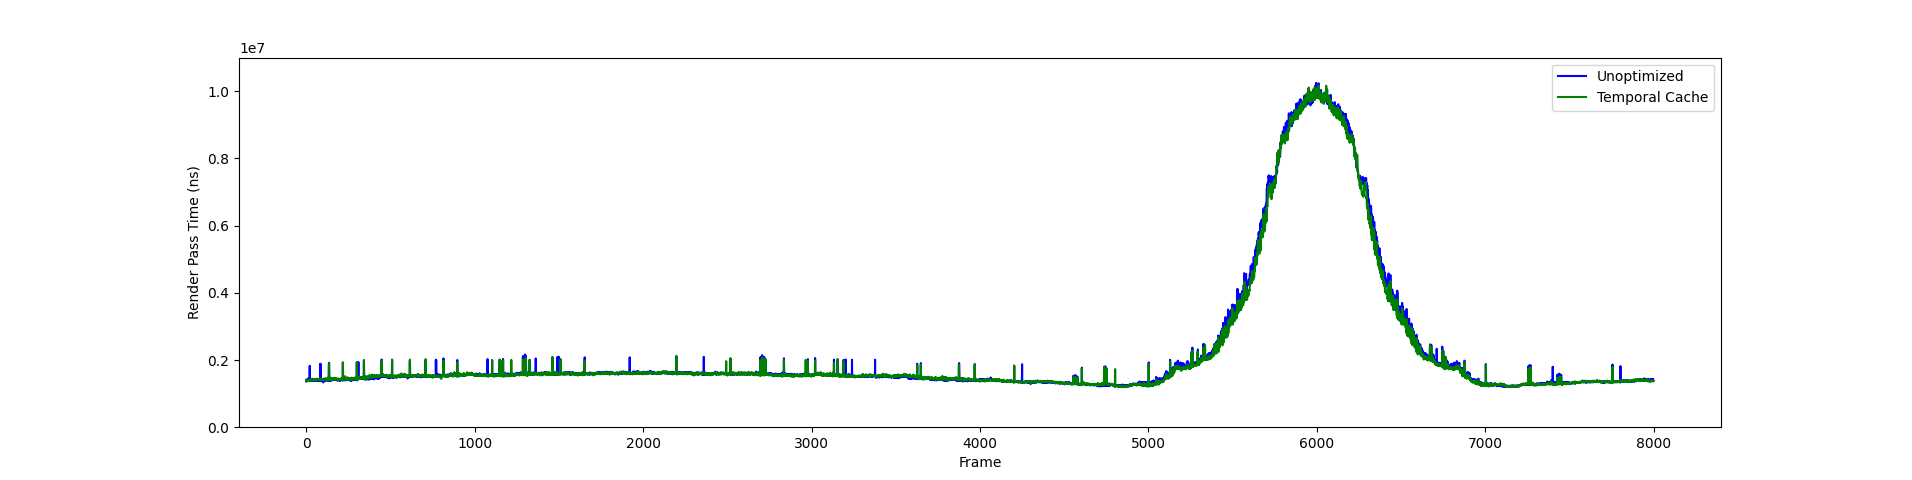
\includegraphics[width=\linewidth, frame]{Images/Results/Mandelbulb-Parameter-Animation.png}
	\caption{A graph showing the performance during an animation of the Mandelbulb parameter, for both unoptimized rendering and rendering using the temporal cache.}
	\label{figure:mandelbulb-parameter-animation}
\end{figure}

Figure \ref{figure:mandelbulb-parameter-animation} shows the graph of the performance over the animation. It is very difficult to see if there are performance differences anywhere in the animation from this, as the two lines overlap almost exactly, but it's useful to know where the performance changes overall during the animation. The fluctuations in the graph are the result of the changing landscape, not outliers. Figure \ref{figure:mandelbulb-parameter-animation-gain} shows a plot of the performance difference over the animation, with a line of best fit plotted to make it clearer (the line of best fit ignores the large spikes in the data).

\begin{figure}[ht]
	\centering
	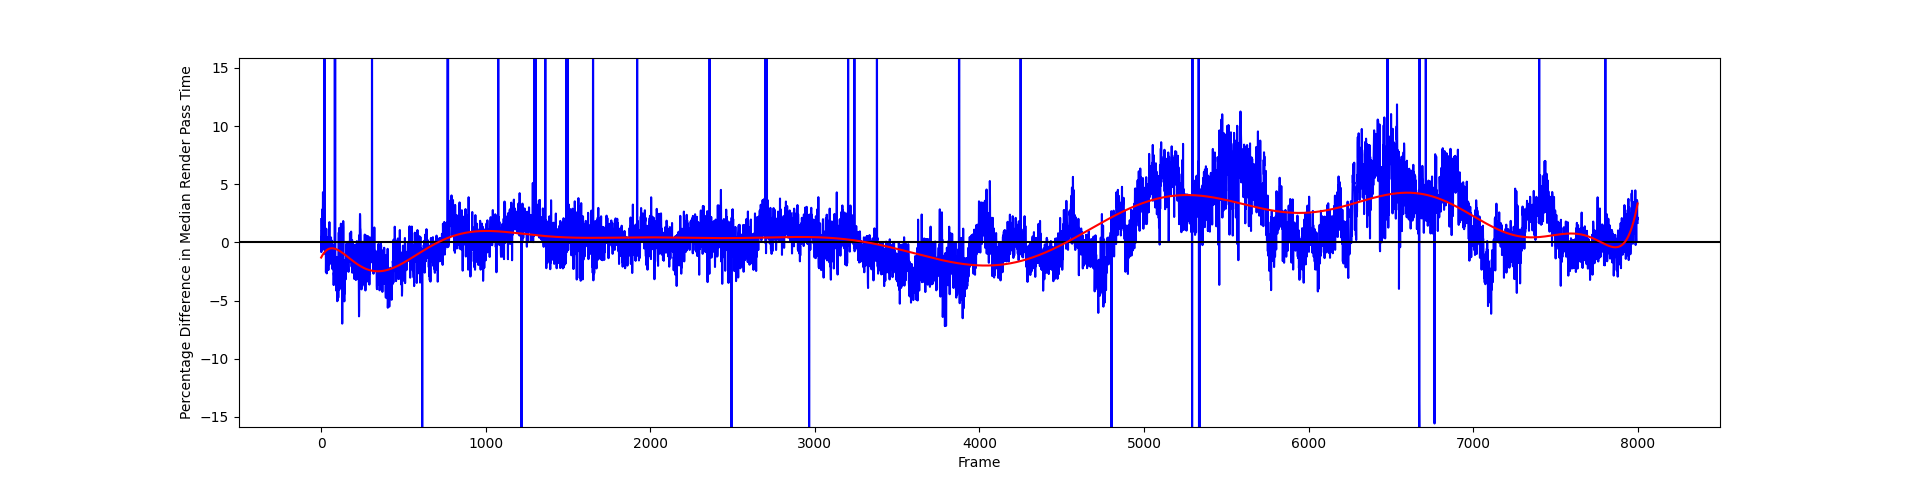
\includegraphics[width=\linewidth, frame]{Images/Results/Mandelbulb-Parameter-Animation-Gain.png}
	\caption{A graph showing the performance difference during an animation of the Mandelbulb parameter, between unoptimized rendering and rendering using the temporal cache.}
	\label{figure:mandelbulb-parameter-animation-gain}
\end{figure}

\subsection{Evaluation}

The main surge in render pass time, in figure \ref{figure:mandelbulb-parameter-animation}, comes about when the parameter is approaching its lowest value. The number of iterations required to reach the surface increases because the surface becomes more intricate. This difference can actually be seen in the image from chapter \ref{chapter:implementation}, figure \ref{figure:mandelbulb-powers}. The image on the left is noticeably darker. This is because the image colouring is done in combination with the ambient occlusion effect described. There is a greater portion of smooth surface, as well as empty space, at this point.\newline

Around the same time as the surge in render pass time, there is a general increase in the performance benefit received from the temporal cache. I believe this is because of the extra smooth surface and empty space, as described. The animation is moving at the same speed, but the changes in the landscape are less from frame to frame. Contrast this with the times around frames 0/8000 and 4000. This is where the parameter reaches 10, which is the starting value. At this point, the landscape is changing the quickest, with new geometry occluding the old at high rates, and less empty space. When the parameter reaches its peak, 16, at frame 2000, these occlusions are still happening, but at a lower rate, so the performance does not dip in the same way as when the animation is at its fastest in terms of occlusion.\newline

Overall the temporal cache performs quite well during the animation, despite, at times, rapid changes in geometry. Additionally, there are more gains than losses, and the losses are smaller than the gains.

\section{Hall of Pillars Static Image Tests}

\subsection{Representative Views}

\begin{figure}[ht]
	\centering

	\begin{subfigure}[c]{0.3\linewidth}
		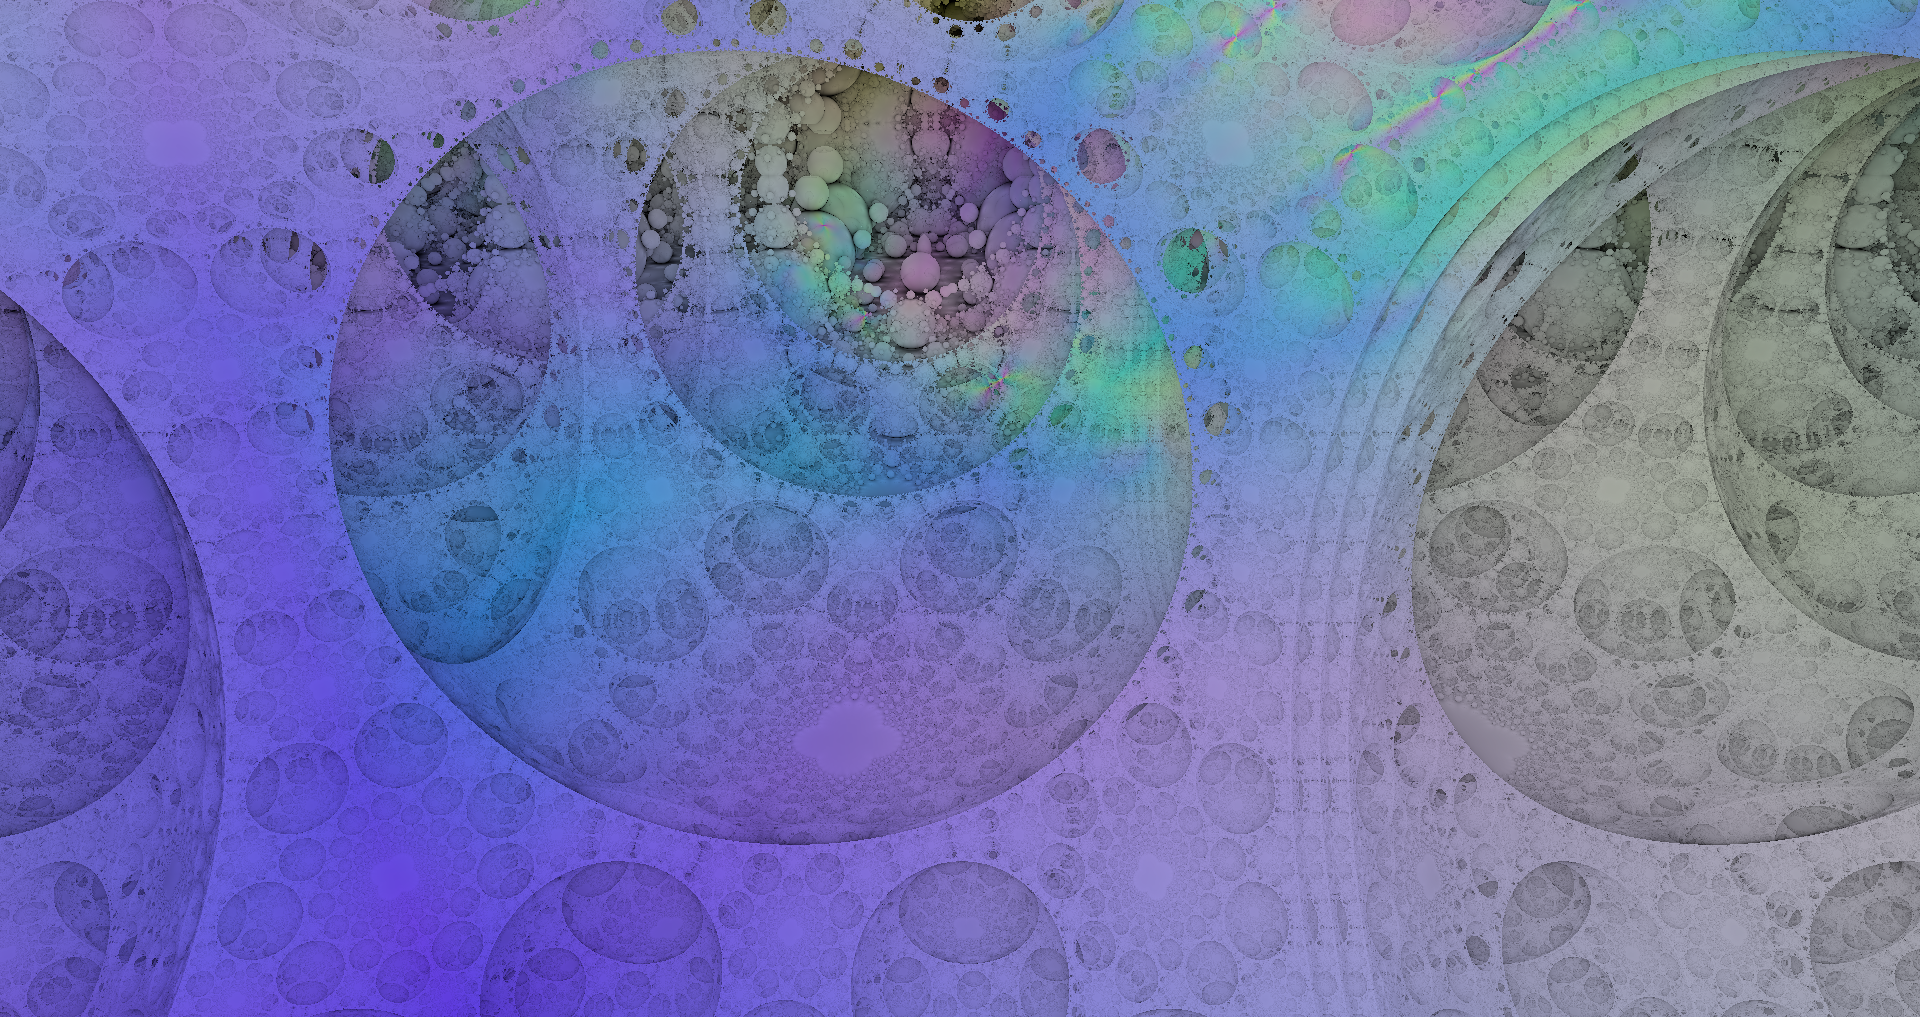
\includegraphics[width=\linewidth, frame]{Images/Results/Hall-Of-Pillars-View-01-Default.png}
		\caption{Hall of Pillars: Default View.}
		\label{figure:hall-of-pillars-view-01-default}
	\end{subfigure}
	\hfill
	\begin{subfigure}[c]{0.3\linewidth}
		\includegraphics[width=\linewidth, frame]{Images/Results/Hall-Of-Pillars-View-02-Large-Hall.png}
		\caption{Hall of Pillars: Large Hall View.}
		\label{figure:hall-of-pillars-view-02-large-hall}
	\end{subfigure}
	\hfill
	\begin{subfigure}[c]{0.3\linewidth}
		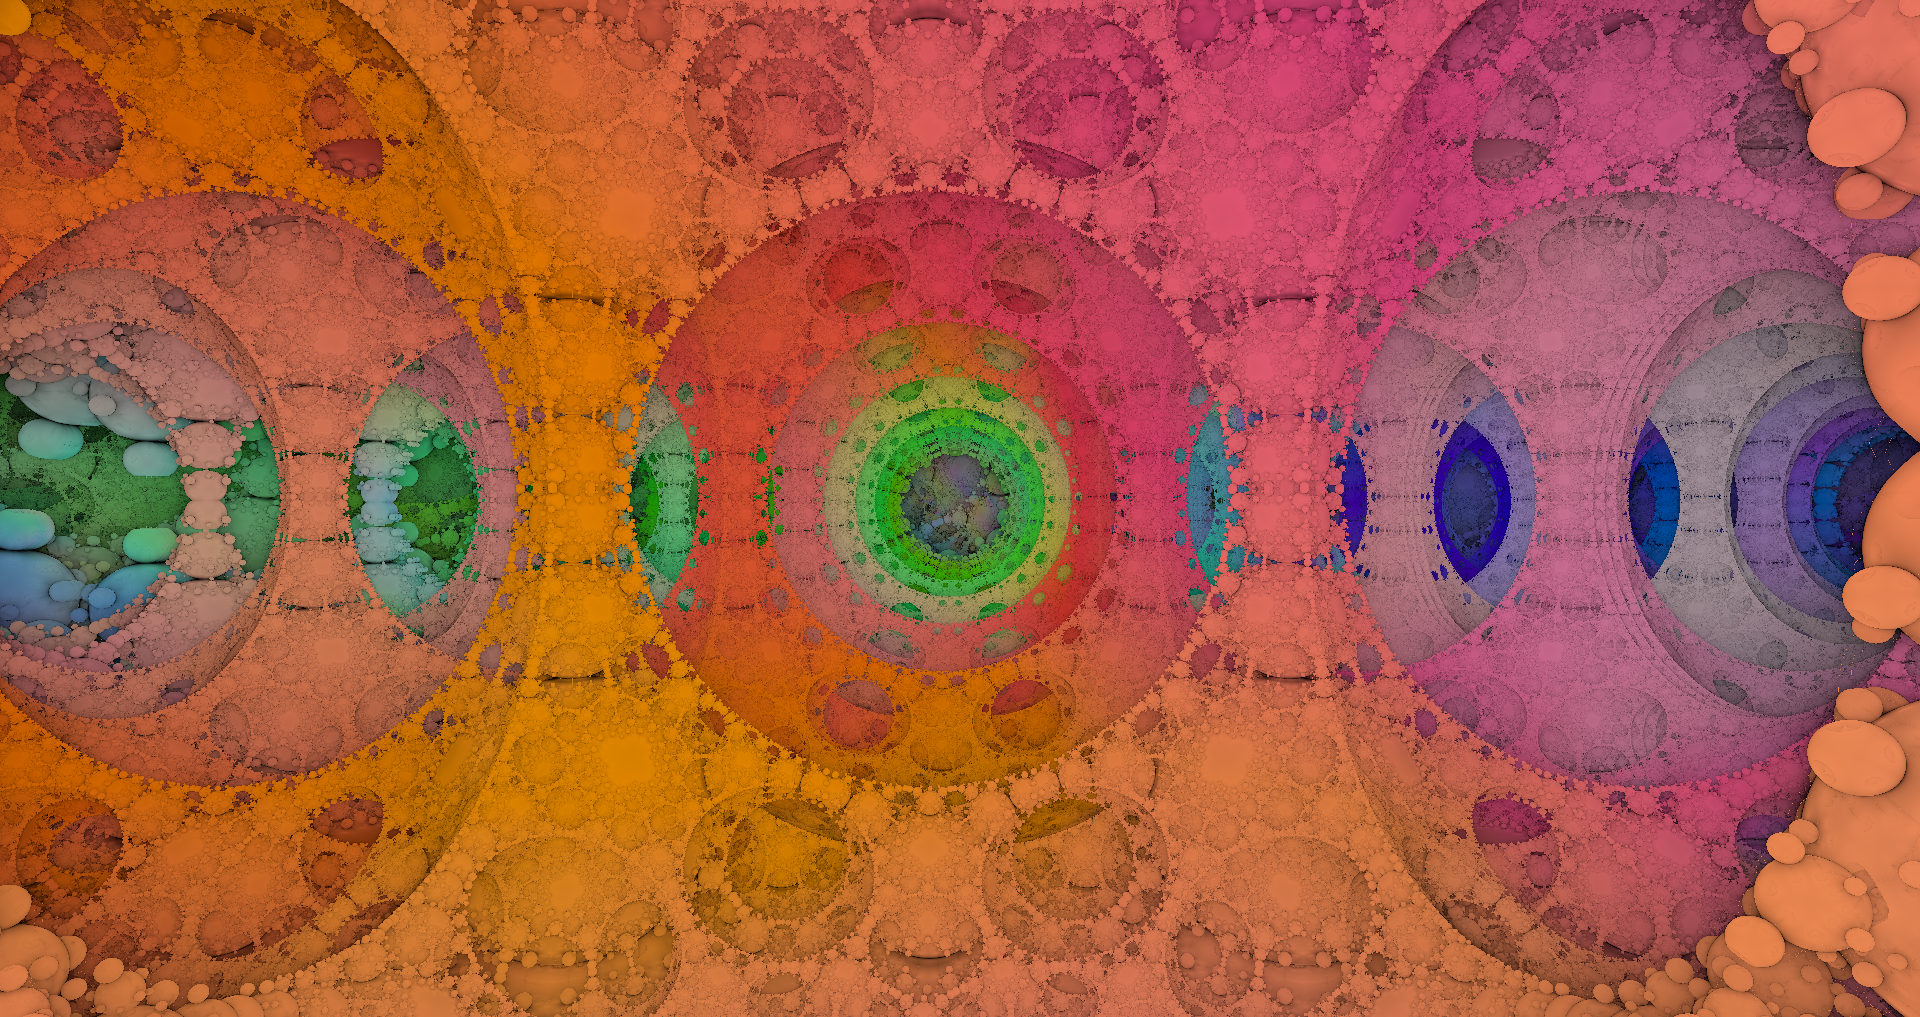
\includegraphics[width=\linewidth, frame]{Images/Results/Hall-Of-Pillars-View-03-Corridor-Of-Bottlenecks.png}
		\caption{Hall of Pillars: Bottleneck Corridor View.}
		\label{figure:hall-of-pillars-view-03-bottleneck-corridor}
	\end{subfigure}
	\hfill
	\begin{subfigure}[c]{0.3\linewidth}
		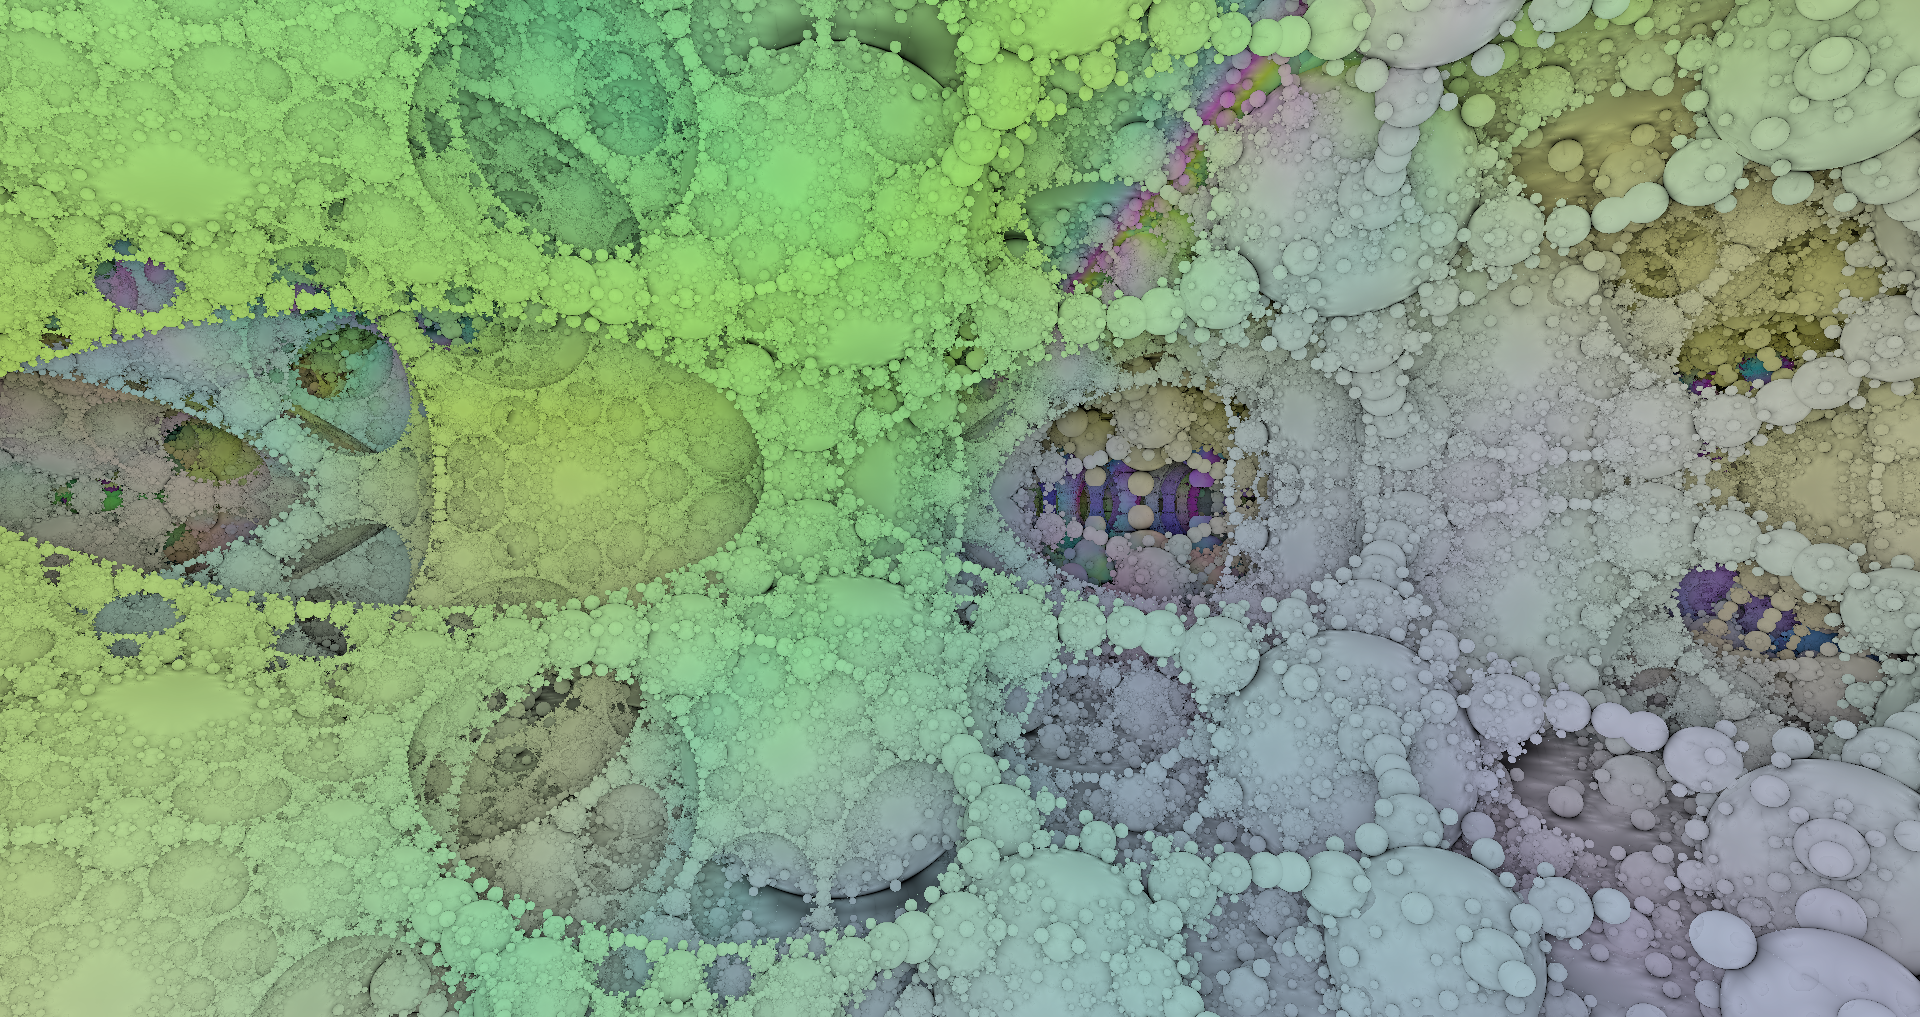
\includegraphics[width=\linewidth, frame]{Images/Results/Hall-Of-Pillars-View-04-Intricate-Geometry.png}
		\caption{Hall of Pillars: Intricate Geometry View.}
		\label{figure:hall-of-pillars-view-04-intricate-geometry}
	\end{subfigure}
	\hfill
	\begin{subfigure}[c]{0.3\linewidth}
		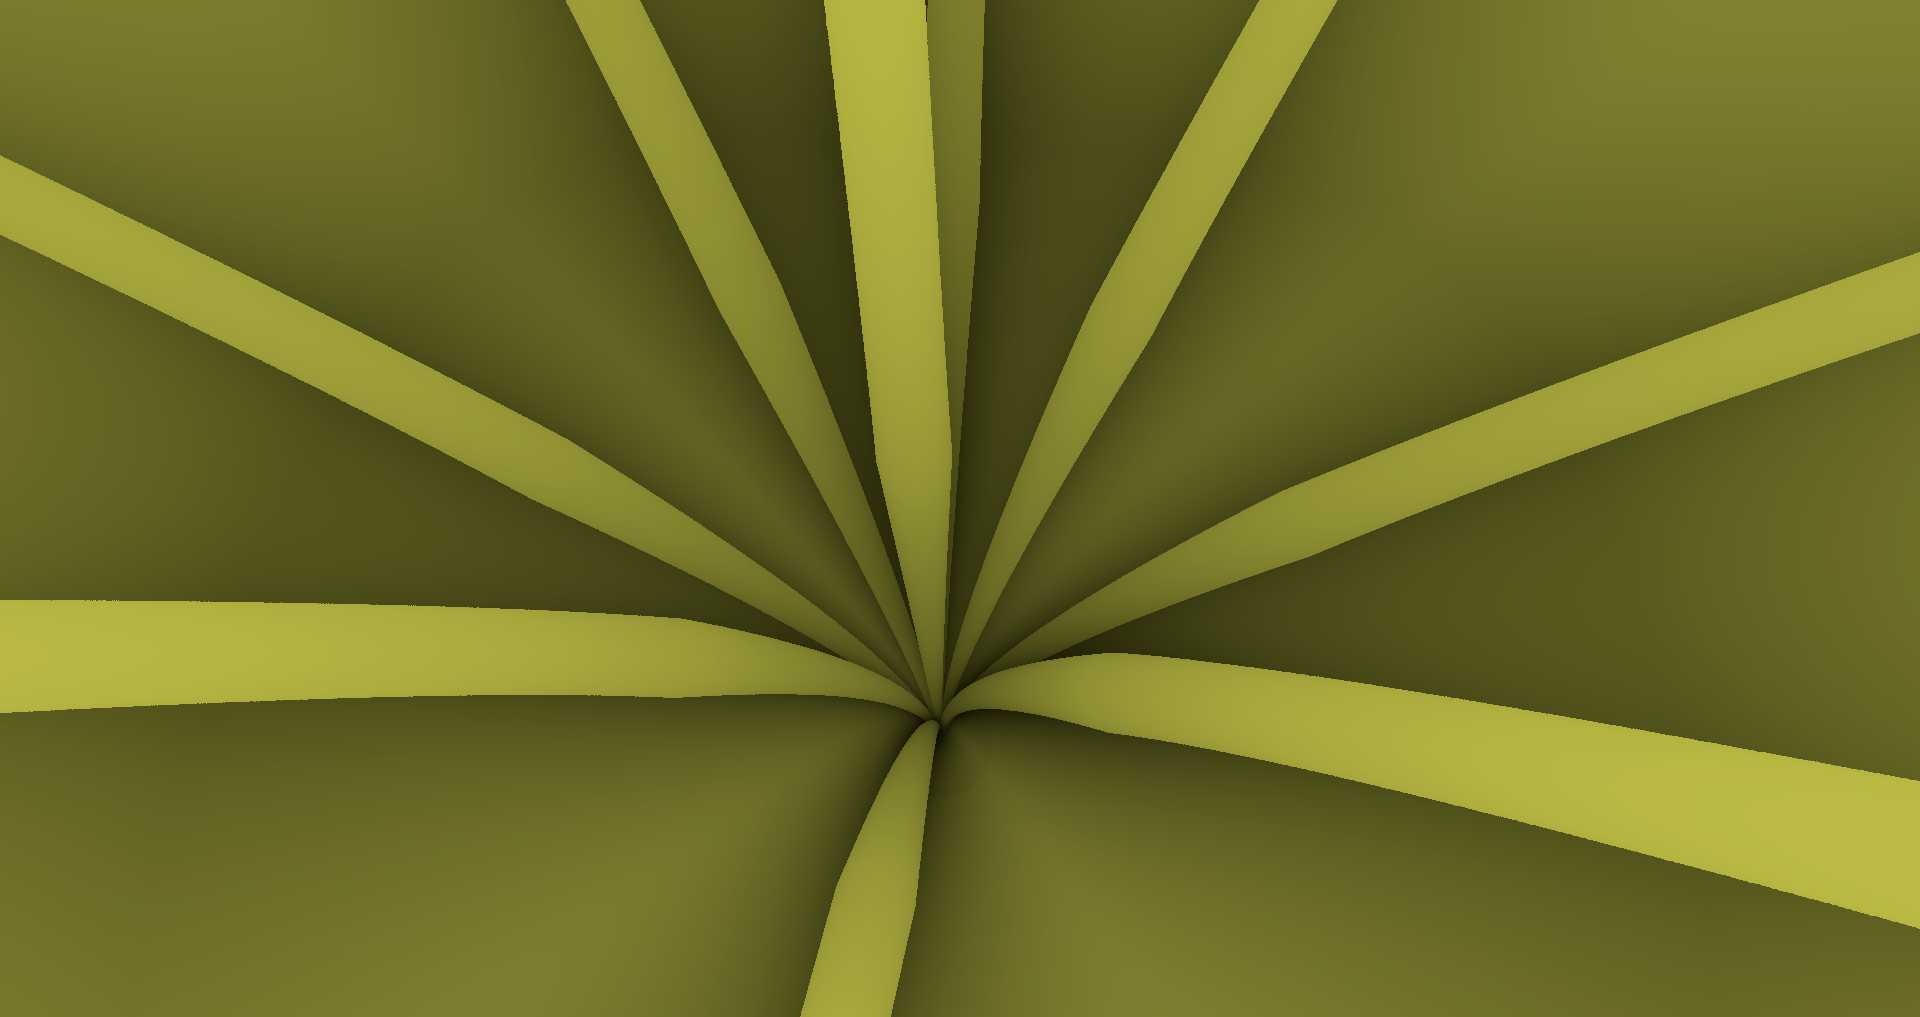
\includegraphics[width=\linewidth, frame]{Images/Results/Hall-Of-Pillars-View-05-Simple-Geometry.png}
		\caption{Hall of Pillars: Simple Geometry View.}
		\label{figure:hall-of-pillars-view-05-simple-geometry}
	\end{subfigure}

	\caption{Five representative views of the Hall of Pillars fractal, used in performance tests.}
	\label{figure:hall-of-pillars-views}
\end{figure}

\subsection{Expected Results}

This fractal contains many bottlenecks (the ray has to pass close to lots of geometry before reaching any surface), so the temporal caching method is expected to perform better here than with the Mandelbulb, in terms of performance difference. A view with very simple geometry was also chosen because of this, as the prediction is that the temporal caching method will provide minimal benefit where these bottlenecks don't exist or the surface is very smooth.\newline

The signed distance field is being used in a somewhat different scenario compared to the Mandelbulb. This fractal doesn't seem to be finite, so only a relatively small area can be covered by the SDF, which makes testing tricky. A ray culling step was tried, to stop any ray which ventures outside the main SDF cube (including in shaders that aren't using the 3D SDF, for consistency) but this did not yield significantly different results to using it as normal, and just allowing the rays to travel outside the box. It was also not representative of the kind of uses for this fractal. Especially in the `Large Hall' view, in which the SDF can only cover a segment of one pillar. I predict that, like with the Mandelbulb, this will not perform well, but judging from the bottleneck view for the Mandelbulb, perhaps it will not perform as badly as it did overall for the Mandelbulb.

\subsection{Results}

\begin{table}[ht]
	\centering
	\begin{tabular}{||p{0.24\linewidth}|p{0.27\linewidth}|p{0.22\linewidth}|p{0.22\linewidth}||}
		\hline
		View & Unoptimized Time (ns) & SDF Difference (\%) & TC Difference (\%)\\
		\hline\hline
		Default & 7524352 & -2.08 & 24.02\\
		\hline
		Large Hall & 12879840 & -1.39 & 12.43\\
		\hline
		Bottleneck Corridor & 10053440 & -10.76 & 26.07\\
		\hline
		Intricate Geometry & 10091680 & -8.04 & 25.62\\
		\hline
		Simple Geometry & 1176352 & -4.76 & 12.39\\
		\hline
	\end{tabular}
	\caption{A table showing the performance differences between the two optimization methods and the base, unoptimized rendering, for five different views of the Hall of Pillars fractal.}
	\label{table:hall-of-pillars-static-results}
\end{table}

As before, table \ref{table:hall-of-pillars-static-results} shows the raw time for the render pass in the unoptimized rendering, as well as performance differences for the SDF and temporal caching (TC) methods.

\subsection{Evaluation}

\subsubsection{Signed Distance Field}

Compared to the Mandelbulb, the SDF performed extremely well, though it still reduced performance in all cases. I think that if the Hall of Pillars distance estimator was more expensive to evaluate, there may have been some positive results. That being said, the SDF was comparatively a lot more coarse than for the Mandelbulb, though it did benefit from an extra subdivision level. I did try changing the subdivision level from 9 to 8, but this did not result in a performance difference.\newline

I think that perhaps for scenes that cross a great deal of the SDF, the shaders are likely to encounter a lot more cache misses, as the total size of the SDF in these tests was 512MB. This will lower performance for scenes such as this. If the subdivision level is too low, and the SDF stretched across too much space, then the voxels will be large, and it will be easier to get past the SDF search stage to fall back on the regular signed distance function. Recall figure \ref{figure:sdf-hybrid-comparison} from chapter \ref{chapter:implementation}. The SDF is clearly a lot more coarse for the Hall of Pillars, in order to cover any kind of decent distance. Another level of subdivision was not possible due to memory constraints. I think this is one reason for the `increase' in performance compared to the Mandelbulb; it simply did not get in the way as much. This is evidenced by the fact that in the view in which it covers the least ground, the Large Hall, we have the smallest performance loss.\newline

Further evidence for this claim is the result for the Bottleneck Corridor view. This view contains a great deal of tunnels and holes in the scene. This view was chosen because I thought it might slow the rays down the most, and therefore result in the greatest performance gain for the temporal cache. It has also resulted in the greatest performance loss for the SDF. The scale of this view means that most of it is contained inside the SDF. This is the worst case out of the views. Lots of bottlenecks, almost all of which are inside the SDF. The Intricate Geometry view has a very similar problem; almost all of that is contained inside the SDF as well (this goes for all views except the Large Hall).\newline

Overall, although the SDF performed better than with the Mandelbulb, I believe this to be an illusion. It is not suitable for use in its current state.

\subsubsection{Temporal Cache}

In contrast to the SDF, the results for the temporal cache were much improved over those it achieved on the Mandelbulb. Even the worst case view resulted in a 12.39\% performance gain. However, this is for a static image, and much of the gain is likely to be lost during movement (more on that in the next section). There isn't much to explain with these results. They are as expected, and likely for the reasons predicted; the presence of a large number of bottlenecks in the scene, and complex geometry. The worst performers were those with less complex geometry (a lot of the Large Hall view was beyond the view distance). For the Large Hall view, I think the performance was lacking partly due to the underestimate of the true distance read from the texture image. A lot of the bottlenecks look like they might have occurred in the last 10\% or so of the ray's journey.\newline

The temporal caching method is particularly well suited to rendering this fractal. The next section will explore how much of the performance gain can be preserved with movement.

\section{Hall of Pillars Animation Tests}

\subsection{Animations}

\subsection{Expected Results}

\subsection{Results}

\subsection{Evaluation}